% Template for 61st conference for non-peer-reviewed articled
\documentclass[convention,e-brief]{aesconf-current}

% Graphics path
\graphicspath{{./}{figures/}}

% UTF-8 encoding is recommended but use one that works for you.
\usepackage[utf8]{inputenc}
\usepackage{pdfsync}
\usepackage{amssymb}

% Highly recommended package for better looking text automatically.
\usepackage{microtype}

% Natbib is used for more control on citations. You can use other moderd
% bibliography packages but please try to match the provided style.
\usepackage[numbers,square]{natbib} 


% These are useful for different purposes.
\usepackage{color}
\usepackage{url}


% The full title of the paper
\title{ Immersive Guitar Playback System Using HRIRs and Spherical Microphone Array Measurement in a Room}

% Put the authors in order here. The number in brackets define the corresponding affiliation.
\author[1]{Takashi Minagawa}
\author[1]{Kazuma Watanabe}

% Affiliations go here
\affil[1]{Graduate School of Design, Kyushu University}



% Correspondece should include the corresponding author's name and e-mail address
\correspondence{Takashi Minagawa}{tmtakashi7@gmail.com}

% These are used for headers. Anything that fits is okay. Please use proper punctuation.

% If there are many authors, please use the form "First author et al."
\lastnames{Minagawa and Watanabe}

% Short title should describe your topic but not be too long.
\shorttitle{Guitar Playback with HRIRs and Spherical Array Signals}


% This is required and draws the top title
% AES top title. A little bit volatile but should work for now.
\savebox{\AEStop}{%
	\begin{minipage}{\textwidth}%
		\rule{\textwidth}{1.5pt}\\%
		\\%
		\begin{minipage}[c][\iftoggle{convention}{3.2cm}{3.7cm}][t]{0\textwidth}%
			\includegraphics[width=20mm]{AESlogo}%
		\end{minipage}%
		\begin{minipage}{\textwidth}%
			\sffamily%
			\begin{center}%
				\LARGE Audio Engineering Society\\%
				\iftoggle{e_brief}{%
				\hspace{3mm}\fontsize{36}{38pt}\selectfont Student Design  \\Competition\\%
				}{%
				\iftoggle{convention}{%
				\fontsize{36}{38pt}\selectfont Convention Paper\\%
				}{%
				\fontsize{36}{38pt}\selectfont Conference Paper\\%
				}}%
				\vspace{0.2cm}%
				\large Presented at the \AESConferenceNumber \iftoggle{convention}{Convention\\}{Conference on\\}%
				\iftoggle{convention}{}{\AESConferenceTopic\\}%
				\AESConferenceDate, \AESConferenceLocation%
			\end{center}%
		\end{minipage}\\%
		\vspace{0.2cm}\\%
%		\begin{minipage}{\textwidth}%
%			\rmfamily\itshape\small%
%		\end{minipage}\\%
%		\\%
		\rule{\textwidth}{1.5pt}%
	\end{minipage}%
}

% Begin document
\begin{document}

\twocolumn[
    \maketitle

    \begin{onecolabstract}
        A guitar playback system with a modern binaural rendering method is proposed.
        The system reproduces the binaural sound image of the sound field produced by a electric guitar loudspeaker cabinet. This system gives immersive guitar playing experience by convolving rendered binaural impulse response with the pre-amplified guitar signal.
        The system was composed from directional impulse responses obtained from a 80-channel spherical microphone array and a HRIR dataset, and integrating them in the spherical harmonic domain.
        This work provides an outlook of the immersive guitar playing experience.
    \end{onecolabstract}
]

\section{Introduction}

Electric guitar players are not always in the best situation to play through a cranked up guitar amplifier, since they need to consider about their housemates and neighbors.
The best known solution of this problem is using a guitar amplifier simulator such as Axe-Fx series by Fractal Audio Systems\footnote{\url{https://www.fractalaudio.com/}} and Kemper Profiler by Kemper Amps\footnote{\url{https://www.kemper-amps.com/}}.
These modern guitar amp simulators reproduces the speaker cabinet section of the amplifiers by convolving the pre-amplified guitar signals with recorded impluse responses of the target cabinets.
While these systems simulates the original amplifiers significantly well, they lack the functionality of reproducing the farfield interaction of speaker cabinets and rooms especially while monitoring on headphones, since those systems focus on reproducing the nearfield response of the original rig system.
In addition, the phantom image of the processed guitar signal is stuck in the center regardless of the player's head position.
The simplest solution to these problem is to apply reverberation and directional cue by convolving room impulse response and HRIR, but a single room impulse response only contains the response of a single point of a room and this approach will completely igonore the interation between directional component of the room sound reflection and the directional cue of HRIRs.
This work aims to overcome these problems by employing directional impulse response signals of a guitar speaker cabinet in a room obtained from a spherical microphone array and HRIR datasets, and combining them in spherical harmonic domain as shown in \cite{Andersson2017-qg}.
The authors implemented a system which reproduces binaural guitar speaker cabinet responses in a room, with a functionality to modify the azimuth of the impulse response rendering direction.

\section{Methods}

\subsection{Theory}
The theory behind the binaural signal rendering process based on \citet{Andersson2017-qg}'s work is briefly described below.
Further details are desribed in \cite{Andersson2017-qg} and they are left to the readers.

The frequency domain signals in the listener's ear postitions $S^{l, r}$ can be desribed as the combination of head-related transfer function (HRTF) $H^{l, r}(\omega, \Omega)$ and plane wave decomposition of the sound field $D(\omega, \Omega)$ as below.

\begin{equation}
    \label{hrtf_pw}
    S^{l, r}=\int_{\mathbb{S}} H^{l, r}(\omega, \Omega) D(\omega, \Omega) d \Omega
\end{equation}

$\omega$ is angular frequency ,$\Omega$ is angle vector $(\varphi, \theta)$ in spherical coordinates, and $\mathbb{S}$ represents a sphere surface.
Plane wave decomposition $D(\omega, \Omega)$ of a sound field can be further described as


\begin{equation}
    D\left(\omega, \Omega\right)=\sum_{n=0}^{\infty} \sum_{m=-n}^{n} d_{n}(k r) P_{n m}(\omega) Y_{n}^{m}\left(\Omega\right)
\end{equation}
, where $P_{nm}$ is spherical harmonic expansion coefficient of the sound field and $Y^{m}_n$ is complex-symmetric spherical harmonics function which can be written as

$$
    Y_{n}^{m}(\varphi, \theta) =(-1)^{m} \sqrt{\frac{2 n+1}{4 \pi} \frac{(n-|m|) !}{(n+|m|) !}} P_{n}^{|m|}(\cos \theta) e^{i m \varphi}
$$
.
In an open sphere and omnidirectional microphone situation, radial function $d_n$ can be written as

$$
    d_{n}(kr)=\frac{1}{4 \pi i^{n} j_{n}\left(k r\right)}
$$
, where $k$ is wave number, $r$ is the radius of the sphere and $j_n$ is spherical bessel function of first kind.

Using $H_{nm}^{l,r}$, the spherical harmonic expansion coefficients of HRTF, and the orthonormality of spherical harmonics, the following equation can be deduced from Eq.\ref{hrtf_pw}. $a_{m}$ is equal to $1$ for all $m$ while comple-symmetric form of spherical harmonics is used.

\begin{equation}
    \label{binaural_signal}
    S^{l, r} =\sum_{n=0}^{\infty} \sum_{m=-n}^{n} d_{n} a_{m} P_{n(-m)} H_{n m}^{l,r}
\end{equation}

In addition, binaural signals with listener's head rotating counter-clockwise in azimuth plane by $\alpha[\mathrm{rad}]$ is given by

\begin{equation}
    \label{rotation}
    S^{l, r}(\alpha)=\sum_{n=0}^{\infty} \sum_{m=-n}^{n} d_{n} a_{m} P_{n(-m)} H_{n m} e^{-j m \alpha}
\end{equation}

\subsection{Measurements and Implementation}

Impulse response of a guitar loudspeaker cabinet (Marshall 1960A) in the reverberation variant room in Kyushu University was measured with 80 channel spherical microphone array as described in Fig.\ref{fig:fullerene}.
The measurement was done by exciting the loudspeaker with swept sine signal, and the horizontal distance between the loudspeaker cabinet and the microphone array was 1.5m.
HRIR\_L2702 dataset by \citet{Bernschutz2013-zy} was used as HRIR database.
Binaural impulse response in each azimuth direction according to Eq.\ref{rotation} are rendered with \emph{sound\_field\_analysis-py} \footnote{\url{https://github.com/AppliedAcousticsChalmers/sound_field_analysis-py}}, a Python package which is based on SOFiA toolbox\cite{Bernschutz2011-rj}.
The impulse responses are then convolved with guitar signal by convolver plugin made by the JUCE\footnote{\url{https://juce.com/}} framework, a plugin framework in written in C++, with a rotation slider GUI which can adjust the rotation angle $\alpha$ as described in Fig.\ref{fig:gui}.

\begin{figure}
    \centering
    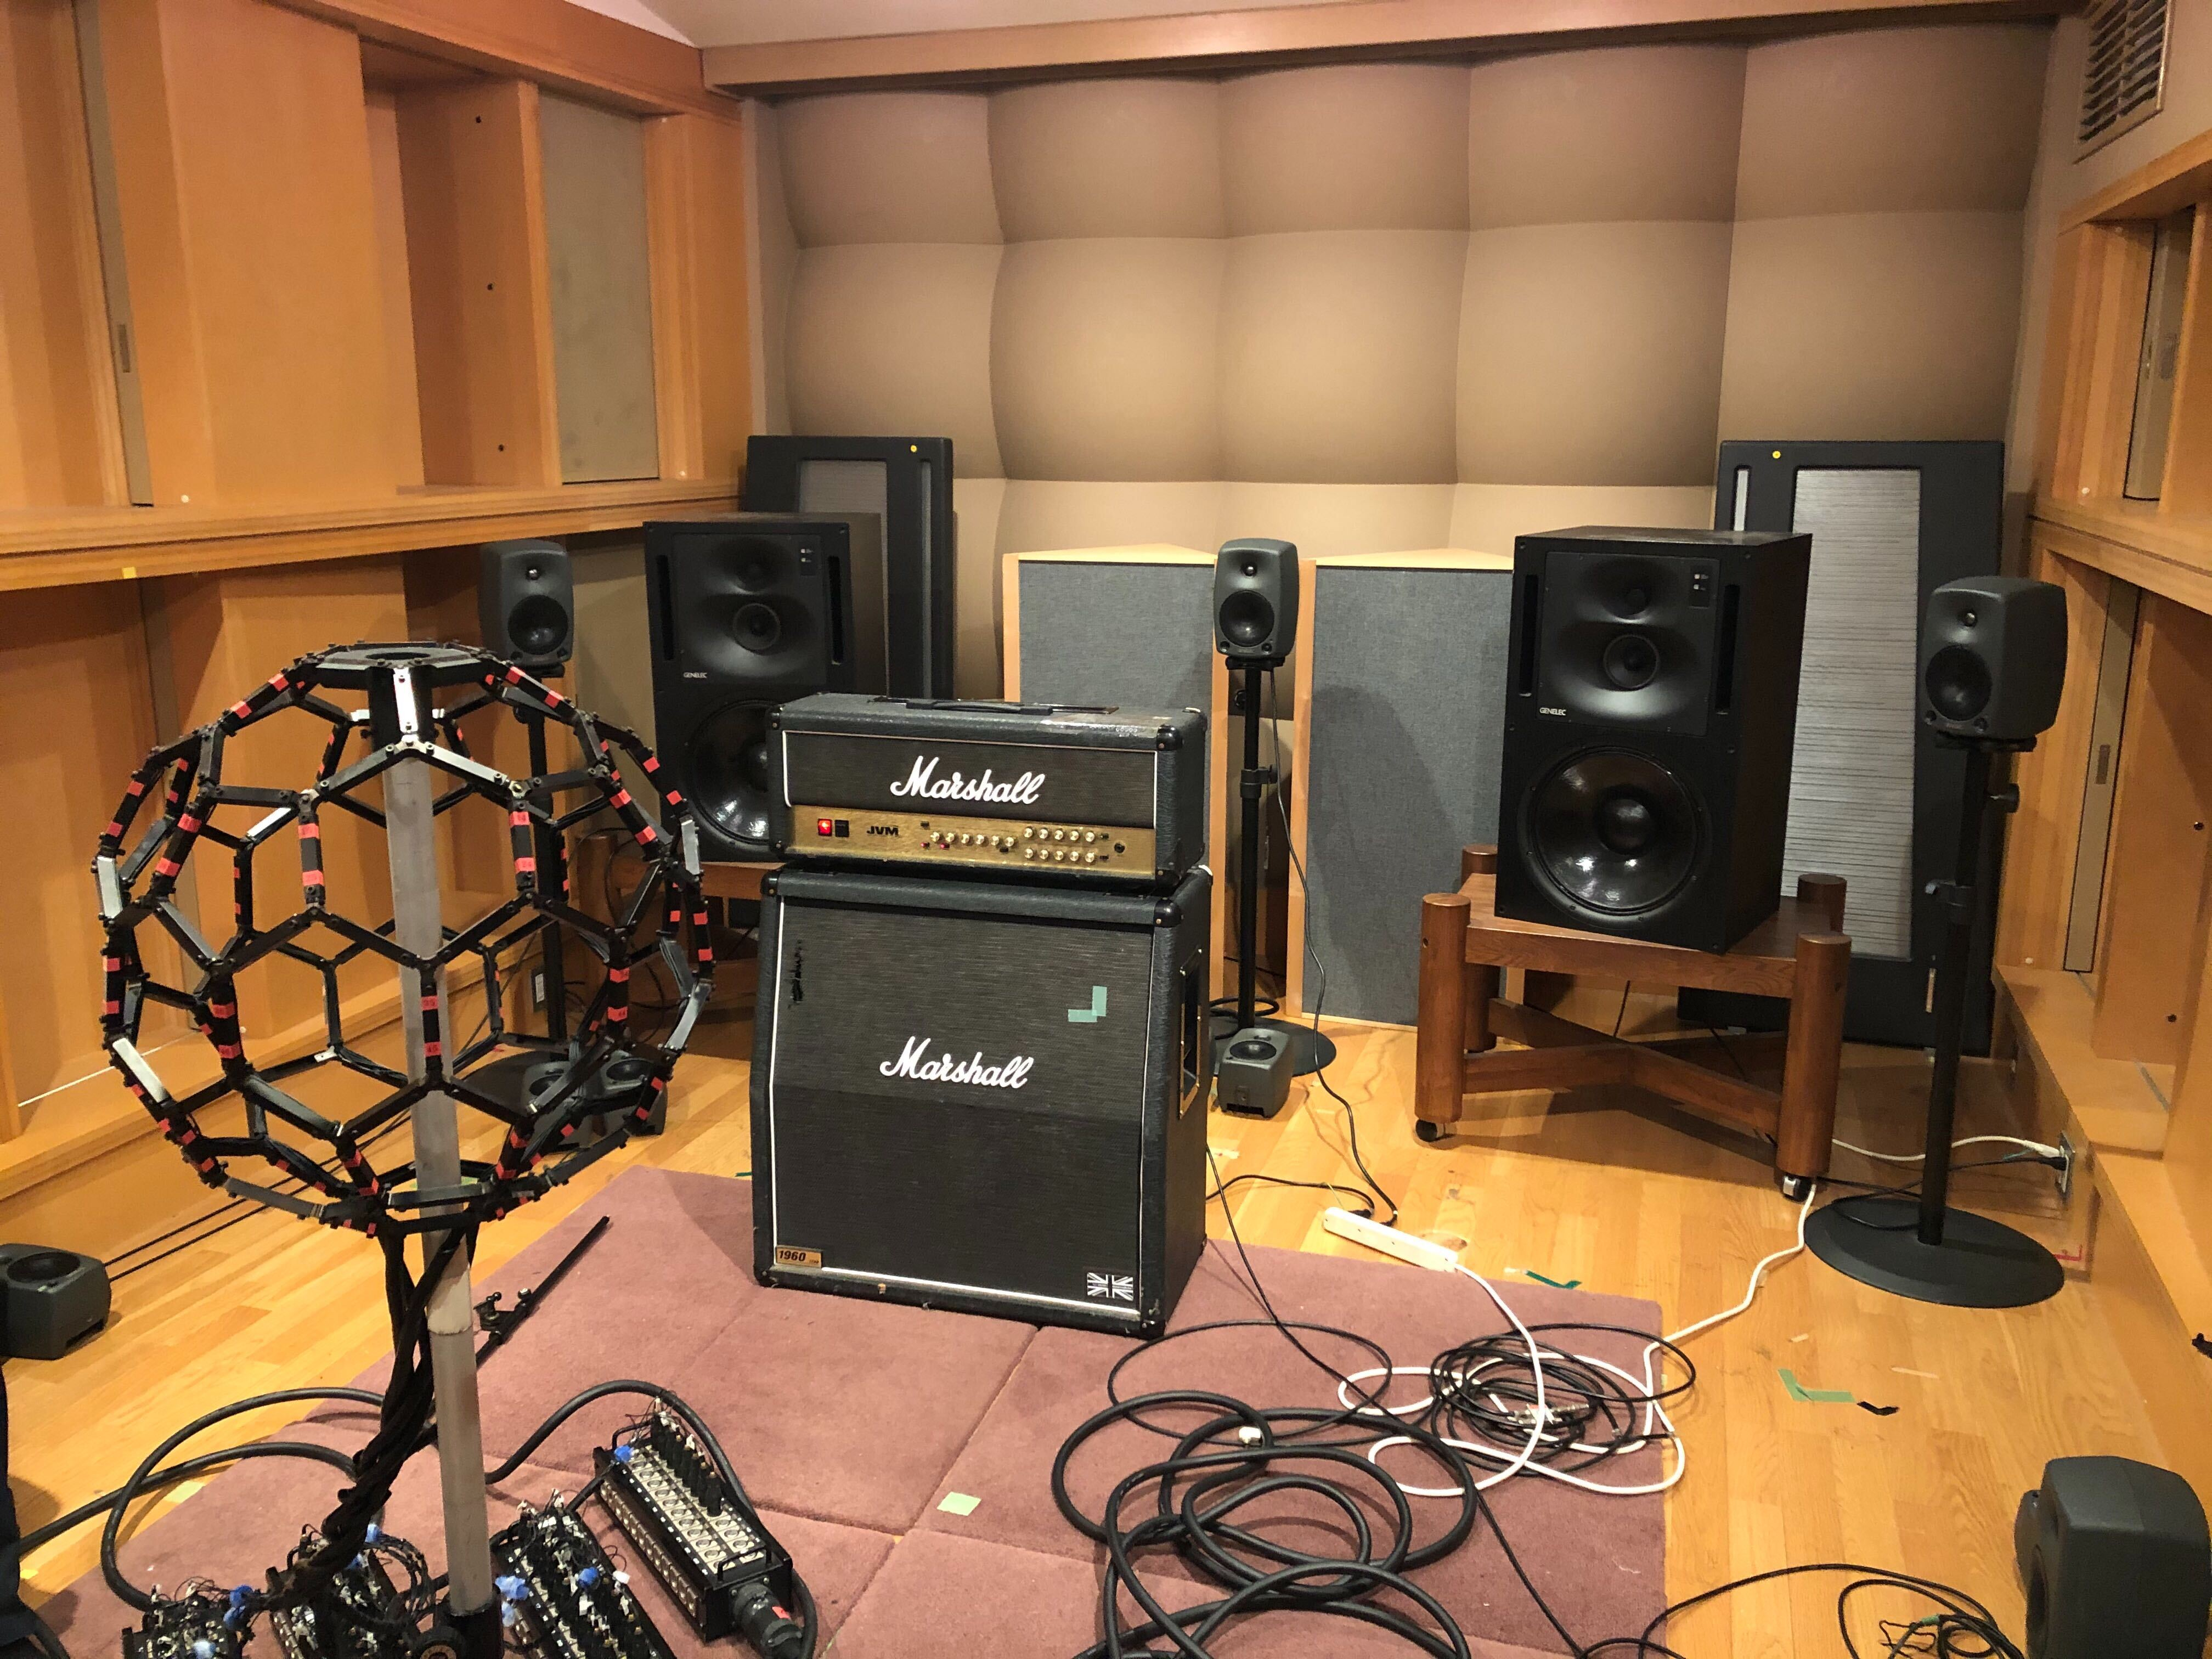
\includegraphics[width=0.45\textwidth]{./fig/fullerene.jpg}
    \caption{Measuring a guitar cabinet impulse response in a room with 80 channel spherical microphone array}
    \label{fig:fullerene}
\end{figure}

\begin{figure}
    \centering
    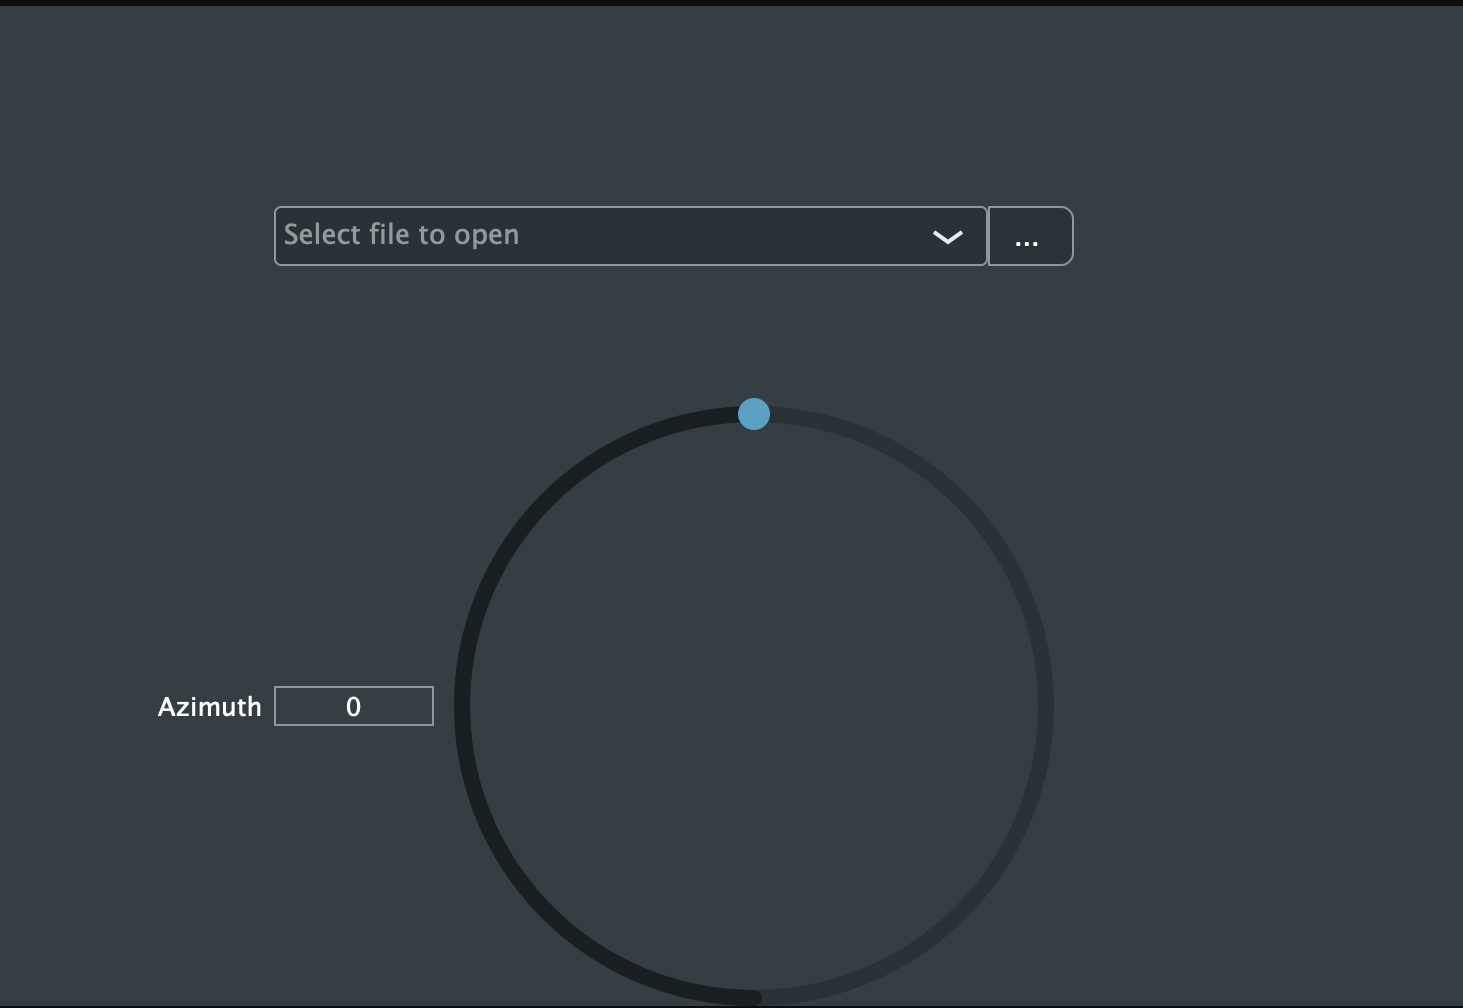
\includegraphics[width=0.45\textwidth]{./fig/gui.png}
    \caption{The GUI of the plugin (prototype)}
    \label{fig:gui}
\end{figure}

\section{Results and Discussion}
With the procedure described, we could successfully implement a guitar loudspeaker cabinet signal reproduction system which renders and convolves impulse responses from a guitar loudspeaker cabinet with the room acoustic response and directional cues from the HRIRs.
However, the following reinforcements to the system are needed to improve the immersive guitar playing experience and they are currently work in progress.

\begin{itemize}
    \item A binaural signal rendering backend within the plugin to dynamically render binaural signals from other directional impulse response and HRIR dataset in SOFA convention format.
    \item Integration of head-tracker to convolve impulse response of the appropriate angle in relation to the listener(player)'s head rotation.
\end{itemize}

\section{Summary}

A guitar loudspeaker cabinet simulation system which reproduces binaural impulse response containing information of directional room acoustic response and directional cues from HRIR was proposed, and its prototype was successfully implemented.
Further improvements are needed to extend the immersive guitar playing experience.
The authors hopes this work broadens the perpective and potentials of applications of binaural rendering technologies and musical signal processing technologies.



\bibliographystyle{jaes}

% Reference to bibliography file.
\bibliography{refs}


\end{document}
